\chapter{Proposed Algorithm}\label{ch:algorithm}
The objective of the human counting algorithm is clarified as following.
 
The detector should be capable of detecting human objects in a relative large range of temperature, because the detected temperature of human body depends heavily on the wearing clothes and individual body condition. The detector should be sensitive to detect a human that is slightly hotter than ambient environment. Meanwhile, fluctuation of the environment temperature should be taken as a reference carefully. A pixel value that is just above the ambient temperature in a cool morning would be regarded as active, but a same value would probably be a noise reading in the afternoon of the same day.

The human body tracker should work properly in single human events, as well as more complicated events when multiple people interact with the door, including but not limited to: two people traversing parallel, traversing sequential but with a narrow distance, traversing in opposite direction, or one person standing still and another pass by. The tracker should not assume that the detected pixel blobs are separated perfectly, and should be able to track two once separate blobs when they merge, as well as assign the correct labels when they split.
\section{Blob Detection}
\subsection{active pixel detection}
Before the actual fore- and background segmentation, an early detection process is conducted on the $8\times8$ coarse image to see whether there is a potential heat source in the camera view. We check if there are at least three pixels having a value $1.5^\circ C$ higher than the room temperature. The parameters are chosen based on the following calculation. When installed at a height of $2.5m$, the Grideye sensor covers an area of about $8m^2$, which is much larger than a human body. However, when a human enters the camera view, the projection of his body on the image is caused by the horizontal plane of the shoulders, which is much higher than the ground and closer to the camera. Assuming the average shoulder height is $1.4m$, the real coverage of the camera is $4m^2$, only half of the ground area that it can cover. We assume the horizontal plane of a human body is no less than $2dm^2$, which amounts to at least three pixels in the image frame. The threshold $1.5^\circ C$ above the room temperature is chosen to filter out the sensor noise, we denote this threshold as $T_{lb}$ (low boundary).
%todo: 大概的示意图
\subsection{the baseline formula}
To separate human objects from the background, we follow the idea of calculating a global threshold from image statistic values, which is inspired by \cite{virtualtrack} and \cite{jeong2014probabilistic}. The threshold $T_{th}$ is calculated by the following formula (\autoref{eq:detectionthreshold}), where Max is the maximum pixel value among all 64 pixels and SD is the standard deviation. By thresholding, the original raster image is linearly interpolated to a resolution of $71\times71$ by inserting nine pixels between each pixel to avoid numeric issues in the following segmentation. The same resolution is also used by \cite{virtualtrack} and \cite{mika}.
\begin{equation}\label{eq:detectionthreshold}
  T_{th} = max\{Max - 4\times SD, T_{lb}\}
\end{equation}

The formula is simple but effective. The result is shown in \autoref{fig:detectioninterpolate}. Comparing image (c) and (e), it is apparent that the interpolation step is necessary to preserve more information from the original image and obtain a smooth shape of the object.
\begin{figure}
  \centering
  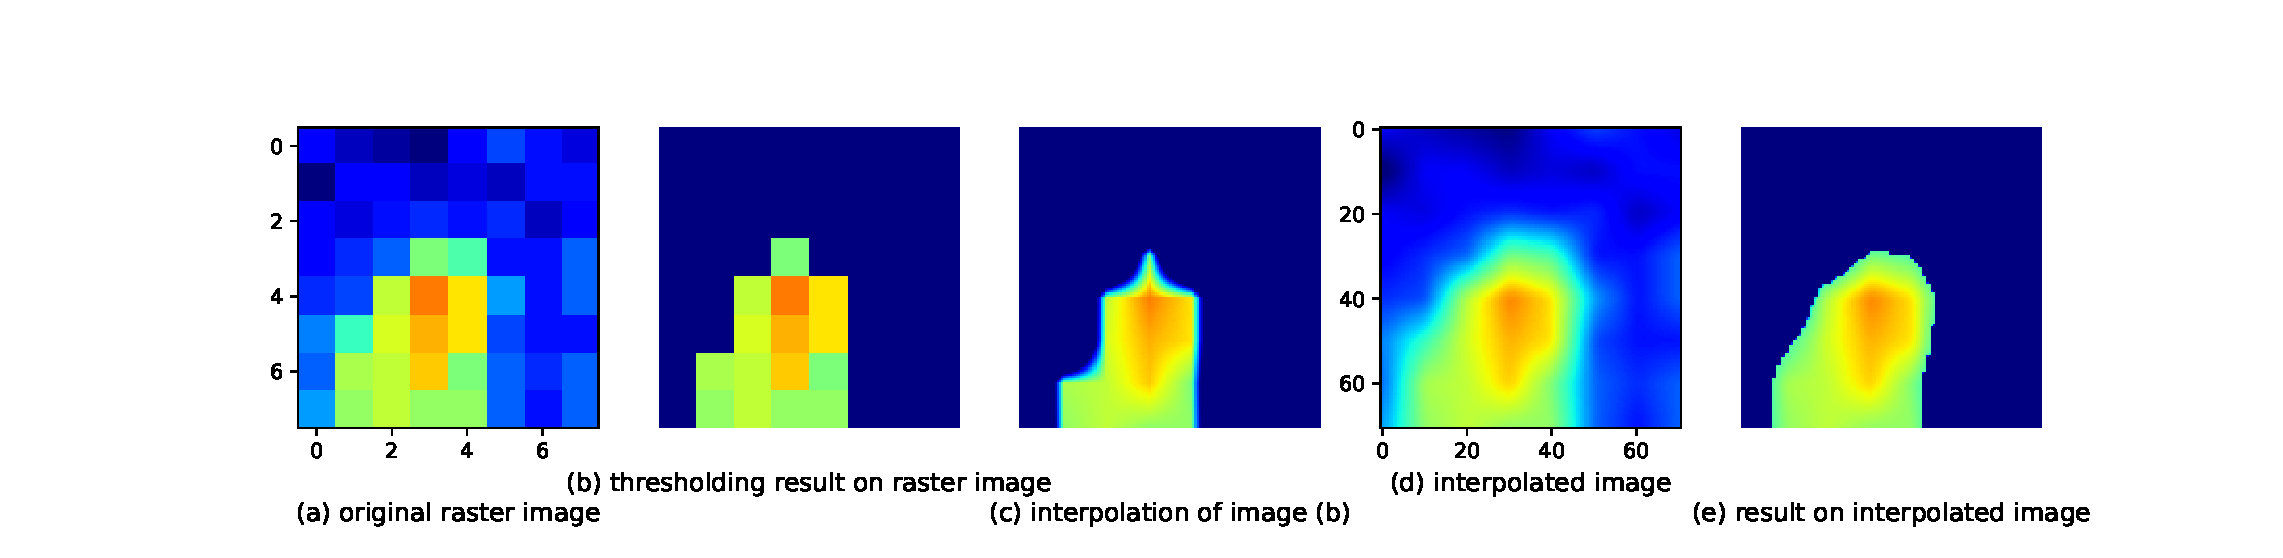
\includegraphics[width=\textwidth]{figures/detect_interpolate.eps}
  \caption{Result given by \autoref{eq:detectionthreshold}, the interpolated image preserves more details after thresholding.}\label{fig:detectioninterpolate}
\end{figure}

\subsection{a spacial filter}
We notice that a single global threshold cannot separate two close objects very well. When two human stand close to each other, the small region between them will have a temperature higher than the room temperature because the pixel value results from a size-weighted average of both objects and background. This effect creates fake active pixels in the binary mask, see the first row in \autoref{fig:detectionspatialfilter}.

Therefore, pixels with hotter pixels nearby should be ignored because they origins from those hotter pixels and do not represent the true heat distribution. Reversely speaking, only those pixels that are hotter than its surrounding, namely local maxima pixels, contain valid information. We use the average filtered image as a spatial filter. After experiments on the collected image frames, a kernel size of 36 is chosen (half of the frame width). The value of every pixel in the filter is calculated by averaging a $36\times36$ neighbourhood surrounding that pixel location in the original image. Afterwards, the original image is compared with the filter pixel-wise, and only those pixels with a value higher than its filter counterpart will be kept. \autoref{fig:detection3d} shows the process in a surface plot, it shows the same image frame from \autoref{fig:detectionspatialfilter}. The threshold calculated from \autoref{eq:detectionthreshold} is applied to the local maxima image. The result is shown in the second row of \autoref{fig:detectionspatialfilter}, it is clear that the bridge connects two objects becomes much narrower. This method outperforms 
\begin{figure}
  \centering
  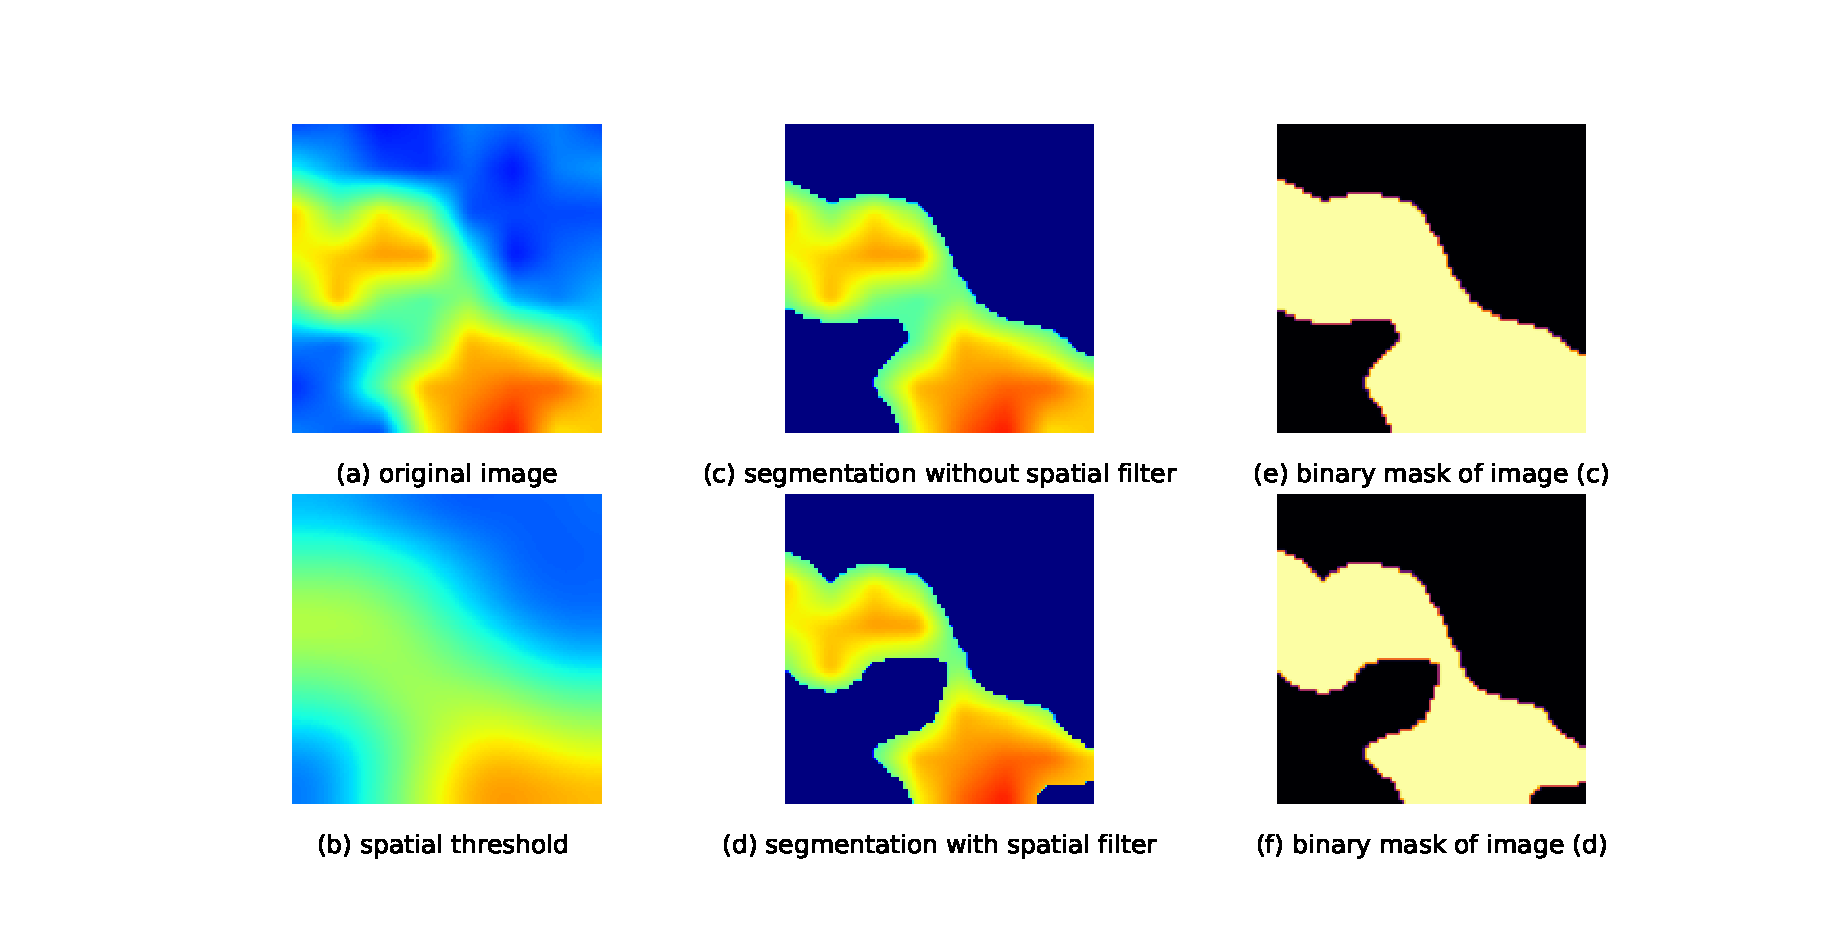
\includegraphics[width=\textwidth]{figures/detect_spatialfilter.eps}
  \caption{After introducing a spatial filter, the region between two objects are no longer marked as occupied.}\label{fig:detectionspatialfilter}
\end{figure}
\begin{figure}
  \centering
  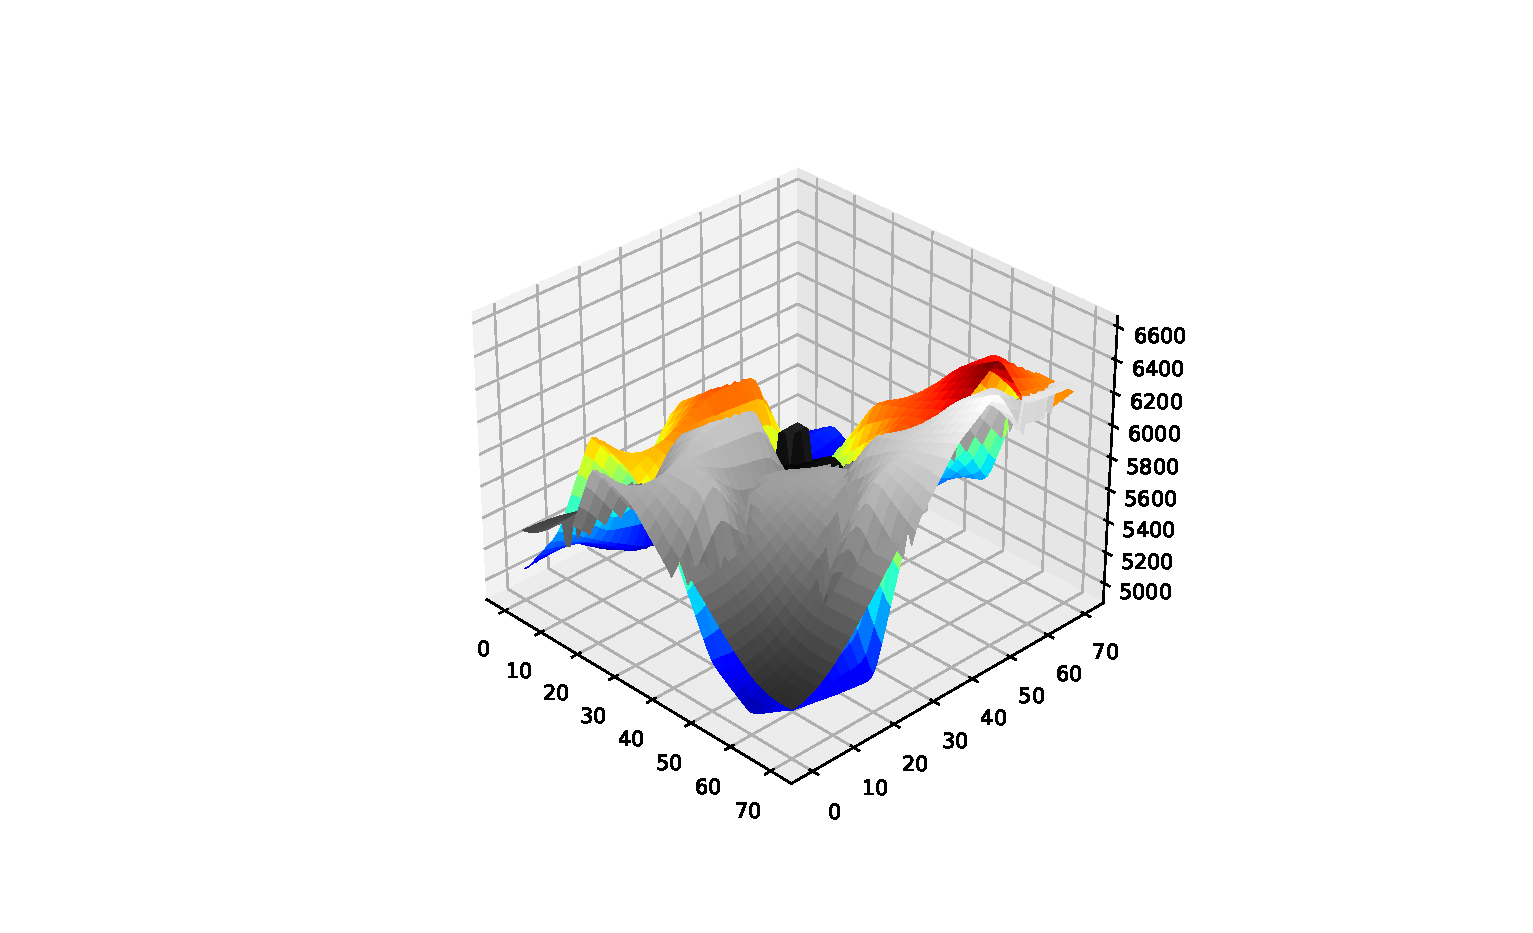
\includegraphics[width=\textwidth]{figures/detect_filterthres.eps}
  \caption{Only those pixels hotter than region average is kept. The gray layer is the average filtered image and the colored layer is the original image.}\label{fig:detection3d}
\end{figure}


\subsection{filling holes}
\section{Feature Extraction}
\section{Human Object Tracking}